% Exemplo de relatório técnico do IC
% Criado por P.J.de Rezende antes do Alvorecer da História.
% Modificado em 97-06-15 e 01-02-26 por J.Stolfi.
% Last edited on 2003-06-07 21:12:18 by stolfi

% modificado em 1o. de outubro de 2008

\documentclass[11pt,twoside]{article}
\usepackage{techrep-ic}
\usepackage[pdftex]{graphicx}
\usepackage{enumerate}

%%% SE USAR INGLÊS, TROQUE AS ATIVAÇÕES DOS DOIS COMANDOS A SEGUIR:
\usepackage[brazil]{babel}
%% \usepackage[english]{babel}

%%% SE USAR CODIFICAÇÃO LATIN1, TROQUE AS ATIVAÇÕES DOS DOIS COMANDOS A
%%% SEGUIR:
%% \usepackage[latin1]{inputenc}
\usepackage[utf8]{inputenc}

\begin{document}

%%% PÁGINA DE CAPA %%%%%%%%%%%%%%%%%%%%%%%%%%%%%%%%%%%%%%%%%%%%%%%
%
% Número do relatório
\TRNumber{45}

% DATA DE PUBLICAÇÃO (PARA A CAPA)
%
\TRYear{10} % Dois dígitos apenas
\TRMonth{05} % Numérico, 01-12

% LISTA DE AUTORES PARA CAPA (sem afiliações).
\TRAuthor{Birocchi, Anderson - RA: 072787 \and Braga, Felipe - RA:070803}

% TÍTULO PARA A CAPA (use \\ para forçar quebras de linha).
\TRTitle{MC823 - Laboratório de Redes\\Projeto 2: Servidor UDP Iterativo para Consulta a Banco de Dados de um Cinema}

\TRMakeCover

%%%%%%%%%%%%%%%%%%%%%%%%%%%%%%%%%%%%%%%%%%%%%%%%%%%%%%%%%%%%%%%%%%%%%%
% O que segue é apenas uma sugestão - sinta-se à vontade para
% usar seu formato predileto, desde que as margens tenham pelo
% menos 25mm nos quatro lados, e o tamanho do fonte seja pelo menos
% 11pt. Certifique-se também de que o título e lista de autores
% estão reproduzidos na íntegra na página 1, a primeira depois da
% página de capa.
%%%%%%%%%%%%%%%%%%%%%%%%%%%%%%%%%%%%%%%%%%%%%%%%%%%%%%%%%%%%%%%%%%%%%%

%%%%%%%%%%%%%%%%%%%%%%%%%%%%%%%%%%%%%%%%%%%%%%%%%%%%%%%%%%%%%%%%%%%%%%
% Nomes de autores ABREVIADOS e titulo ABREVIADO,
% para cabeçalhos em cada página.
%
\markboth{Birocchi, Braga}{MC823 - Projeto 2, Aplicação UDP}
\pagestyle{myheadings}

%%%%%%%%%%%%%%%%%%%%%%%%%%%%%%%%%%%%%%%%%%%%%%%%%%%%%%%%%%%%%%%%%%%%%%
% TÍTULO e NOMES DOS AUTORES, completos, para a página 1.
% Use "\\" para quebrar linhas, "\and" para separar autores.
%
\title{MC823 - Projeto 2, Servidor UDP Iterativo para Consulta a Banco de Dados de um Cinema}

\author{Anderson Birocchi, Felipe Braga}

\date{}

\newpage
\tableofcontents
\newpage

\maketitle

%%%%%%%%%%%%%%%%%%%%%%%%%%%%%%%%%%%%%%%%%%%%%%%%%%%%%%%%%%%%%%%%%%%%%%

\newenvironment{codelisting}
{\begin{list}{}{
\setlength{\leftmargin}{1em}
}
\item\scriptsize\bfseries}{\end{list}}


\begin{abstract}
Complementarmente ao anterior, o objetivo deste projeto é dar uma noção dos aspectos da implementação de um sistema que utiliza comunicação em rede. Desta vez, no entanto, foi usado o protocolo da camada de transporte UDP - \textit{User Datagram Protocol}. Procurou-se verificar as brechas geradas pela inconfiabilidade na entrega deste protocolo, assim como comparar a aplicação com a anterior, em TCP (tanto com relação à implementação como ao desempenho).
\end{abstract}

\section{Introdução}

Vimos no projeto anterior que os sockets TCP são ótimos para atividades que requerem robustez e segurança, como transações bancárias, armazenamento remoto de dados, transferência de arquivos em geral, etc. Porém, em troca dessa robustez e segurança, a velocidade da transmissão é prejudicada, já que no protocolo TCP há controle de fluxo, controle de congestionamento da rede e tratamento de perda de pacotes. Isso não costuma ser um problemas para as atividades citadas anteriormente, pois a velocidade não é algo crucial, no entanto, e se a atividade for uma transmissão ao vivo pela internet? A velocidade é fundamental, e a perda de alguns pacotes não condenam totalmente a transmissão.\\
Para esse e muitos outros casos, são utilizados sockets UDP, com comunicação sem conexão, apenas através de datagramas, que por não ter nenhum tipo de controle de fluxo, congestionamento ou perda de pacotes, consegue uma transmissão rápida porém não confiável de datagramas.\\
E se utilizarmos sockets UDP para o servidor de banco de dados de um cinema já implementado anteriormente? Será que a velocidade de comunicação realmente vai aumentar? Será que a perda de pacotes vai inviabilizar o uso da aplicação?\\
Nosso projeto irá reimplementar o servidor para consultas em bancos de dados de um cinema, mas agora utilizando sockets UDP na comunicação entre o servidor e o cliente.\\
A seção 2 irá especificar novamente o que exatamente o programa deve fazer; a seção 3 irá comentar mais detalhadamente a implementação, as definições, suposições tomadas e ferramentas utilizadas; a seção 4 irá analisar o desempenho da aplicação atraveś de várias medidas de tempo e também uma comparação dos tempos se utilizando TCP e UDP; a seção 5 irá mostrar quão não-confiável inconsistente é a aplicação se utilizando UDP; na seção 6 encontra-se uma breve conclusão sobre o projeto e, por último, na seção 6 estará o código fonte necessário para compilar e executar o servidor e o cliente.


\section{Casos de Uso}

Relembrando o que a aplicação deve fazer, segue abaixo uma listagem de 6 ações que serão implementadas. Nota: as ações com (*) precisam receber um identificador numérico do filme como entrada.\\
As ações sempre serão tomadas pelo cliente, sendo o servidor apenas quem irá processar o pedido. O resultado da ação apenas é vista pelo cliente que a iniciou, deixando o servidor totalmente à parte do que está acontecendo do lado dos seus clientes.
\subsection{Listar todas as informações de todos os filmes}
Mostrar o ID, título, sinopse, horário das sessões e as salas de todos os filmes cadastrados no banco de dados do servidor.
\subsection{Listar ID e título de todos os filmes}
Fazer uma busca rápida de todos os títulos e seus IDs, mais utilizado para auxiliar em futuras consultas, e utilização dos próximos casos de uso.
\subsection{Listar todas as informações de um filme (*)}
Buscar todas as informações sobre o filme com o dado ID.
\subsection{Mostrar a sinopse de um filme (*)}
Mostrar a sinopse completa do filme com o dado ID.
\subsection{Mostrar a avaliação de um filme (*)}
Mostrar a quantidade de votos o filme teve e qual foi a pontuação obtida.
\subsection{Avaliar um filme (*)}
Dar uma pontuação ao filme com o dado ID.



\section{Implementação}
Assim como no projeto anterior, o programa é desenvolvido na linguagem C e utiliza as bibliotecas padrão de comunicação do Unix. Desta vez, porém, são setadas as informações para o uso do UDP (\textit{DATAGRAM\_SOCKET}).\\
O funcionamento básico do sistema é: o cliente envia uma requisição ao servidor, que realiza alguma tarefa (caso necessário) e envia uma resposta ao cliente. Adiantamos que, diferentemente do TCP, a requisição é única, já contendo todas as informações que o servidor possa precisar.\\
No fim, a quantidade de linhas de código de todos os arquivos do sistema (*.c e *.h) é 1246 (aproximadamente 200 linhas a menos que com o TCP - essa diferença se deve às simplicidades geradas pela falta de complexidade do UDP, como será explicado posteriormente).\\
A seguir, serão pontuadas características do desenvolvimento em alguns assuntos que encontramos.\\

\subsection{Dados}
A forma como o sistema armazena os dados, tanto na camada de persistência (arquivo) como na de manipulação (memória) é exatamente a mesma que no primeiro projeto, de modo que o código necessário para a definição e manipulação dos dados foi reutilizado.\\
No entanto, é importante ressaltar que nem tudo que implementamos para o projeto usando TCP foi usado. A explicação disso é que, por causa do caráter de fluxo (\textit{streamming}) do TCP, e para minimizar disperdícios, as mensagens eram sempre enviadas como sequencias de caracteres, e era utilizado um caractere para sinalizar o fim da string. No caso do UDP, a comunicação é baseada em datagramas, e para cada registro que é enviado, um bloco de tamanho fixo é utilizado para comportar os dados do filme. Assim, apesar do desperdício de memória e de bytes sendo enviados pela rede, esta parte da implementação ficou consideravelmente mais simples, pela ausência da necessidade de tratamento do fim do fluxo.\\

\subsection{Protocolo de comunicação usando UDP}
Como o UDP não garante que os dados enviados serão recebidos, e se recebidos, podem chegar fora de ordem, foram implementada duas principais medidas para reger a comunicação:
\subsubsection{Do cliente para o servidor}
Anteriormente, com o uso do TCP, o cliente selecionava a opção, que era enviada ao servidor. No caso de se tratar de uma opção que requer um id, o cliente então lê e envia este id, enquanto no lado servidor a thread responsável por aquela conexão espera este id. O mesmo acontecia para a opção 6, que requer uma nota para avaliar o filme.\\
Como não há uma conexão de fato, seria pouco seguro continuar usando esta abordagem, uma vez que um cliente C1 poderia enviar uma opção que requer um id; e quando o servidor passasse a esperar pelo id, outro cliente C2 poderia enviar uma opção (que seria lida como id), e o programa ficaria inconsistente.\\
É possível pensar na comunicação do cliente com o servidor como uma pergunta e resposta, onde o cliente envia uma pergunta "atômica" (apenas um datagrama), de modo que o servidor sabe exatamente o que o cliente quer com apenas uma mensagem.\\
Para isso, foram empacotadas as informações: \textit{opção}, \textit{id} e \textit{nota} num vetor chamado \textit{request}, mesmo para as opções que não requerem id e/ou nota. O envio deste vetor é, então, a considerada pergunta "atômica" e suficiente.
\subsubsection{Do servidor para o cliente}
Depois de enviar uma pergunta ao servidor, o cliente passa a esperar pela resposta. Mas e se a resposta começar a demorar? O UDP não garante que as mensagens enviadas serão recebidas. Logo, tanto a pergunta como a resposta podem se perder. Assim, no caso de um ou outro, o cliente ficaria bloqueado infinitamente no \textit{recv()}, o que não é interessante.\\
Para contornar isso, implementamos um \textit{time-out} para o recebimento de respostas pelo cliente. Seu funcionamento se dá como segue:\\
\textbf{Ideia 1}\\
Toda vez que o cliente for receber uma resposta do servidor, entra num laço \textit{for()}, razoavelmente grande (por exemplo, de 1000 vezes). A cada iteração, é chamado o \textit{recv()} no modo não-bloqueante (a partir da configuração pela flag). Caso esse \textit{recv()} leia a resposta, sai do laço e sabe-se que nenhuma msg se perdeu. Caso contrário, é chamada uma função de espera \textit{sleep()}, de algum tempo curto (p.e, 100 micro-segundos) e terminado isso, volta ao início do laço. Caso o laço se encerre, sabe-se que a resposta não chegou até o \textit{time-out} e provavelmente ou a pergunta ou a resposta se perdeu.\\
No entanto, ao tentarmos efetuar a implementação, surgiram alguns problemas para conseguir fazer com o que o \textit{recv()} ficasse efetivamente não bloqueante. Tentou-se mudar todo o socket do cliente para não bloqueante, com a função \textit{fcntl()}, que também se mostrou ineficiente. Somado ao fato de este ser um método que faz o processo cliente ficar em espera ocupada (consumindo recursos do processador), optamos por implementar usando a função \textit{select()}.
\textbf{Ideia 2}\\
Dando uma grande facilidade, a função \textit{select()} implementa tanto um "ouvinte" para o socket de leitura, retornando quando algum datagrama chegou até ele, como o \textit{time-out}, tornando a codificação bem mais simples.\\

\subsection{Servidor iterativo X Servidor concorrente}
Em uma aplicação UDP não faz sentido se falar de múltiplas conexões, de concorrência ou de exclusão mútua, pois primeiro, não há conexão, o servidor é iterativo, ou seja, ao chegar um datagrama ele processa e responde ao cliente que pediu, e caso datagramas de outros clientes cheguem no socket UDP, estes ficam numa fila esperando o socket ficar livre novamente; e segundo, por ser iterativo, o servidor não vai permitir que dois ou mais clientes acessem ao mesmo tempo o banco de dados, evitando assim, concorrência e a necessidade de se garantir exclusão mútua.\\


\section{Análise de Tempo}
Para a análise de tempo, foi considerada apenas uma operação a ser analisada,o tempo de consulta ao servidor, já que o tempo de conexão (RTT) não faz mais sentido exatamente por não haver mais conexão.\\
Para se obter uma boa precisão, foi utilizada a função "gettimeofday", que tem a precisão em microsegundos, o que já é boa o suficiente para nossa aplicação. A função pega o tempo atual em que foi chamada, portanto, para calcular o tempo de alguma operação, basta calcular o tempo antes e depois da operação e calcular a diferença entre eles.\\
Foram usadas duas configurações:\\
\textbf{Configuração 1: }Dois computadores presentes na mesma sub-rede (SIFEEC).\\
IP local: 143.106.150.77\\
IP remoto: 143.106.150.74\\
\textbf{Configuração 2: }Um computador no laboratório do IC3 e outro no SIFEEC.\\
IP local: 143.106.150.77\\
IP remoto: 143.106.16.163 (xaveco)\\
\begin{verbatim}
[ra072787@xaveco ~]$ traceroute 143.106.150.74
traceroute to 143.106.150.74 (143.106.150.74), 30 hops max, 60 byte packets
 1  routeric3.lab.ic.unicamp.br (143.106.16.148)  2.801 ms  5.398 ms  7.873 ms
 2  143.106.16.150 (143.106.16.150)  0.099 ms  0.074 ms  0.065 ms
 3  143.106.7.129 (143.106.7.129)  0.218 ms  0.182 ms  0.159 ms
 4  area3-gw.unicamp.br (143.106.1.129)  0.570 ms  0.748 ms  0.981 ms
 5  ptp-nct-nbs.unicamp.br (143.106.199.13)  0.636 ms  0.870 ms  1.036 ms
 6  fee-gw.unicamp.br (143.106.1.10)  1.049 ms  1.332 ms  1.305 ms
 7  le20-10.grad.fee.unicamp.br (143.106.150.74)  2.070 ms  2.047 ms  2.401 ms
[ra072787@xaveco ~]$
\end{verbatim}
\textit{Observação: }Todos os tempos que serão mostrados nas próximas seções estão em micro-segundos, e pode-se verificar todos os valores encontrados na seção de Anexos.\\

\subsection{Tempo de Consulta}
Tempo decorrido entre o cliente realizar o caso de uso 1 (consulta completa de todos os filmes do banco de dados).\\
\textbf{Configuração 1: }\\
Média do tempo de consulta: \textbf{2288,52 us}\\
Desvio padrão: \textbf{792,62 us}\\
\textbf{Configuração 2: }\\
Média do tempo de consulta: \textbf{3606,54 us}\\
Desvio padrão: \textbf{1094,37 us}\\
\begin{figure}[htb]
  \centering
  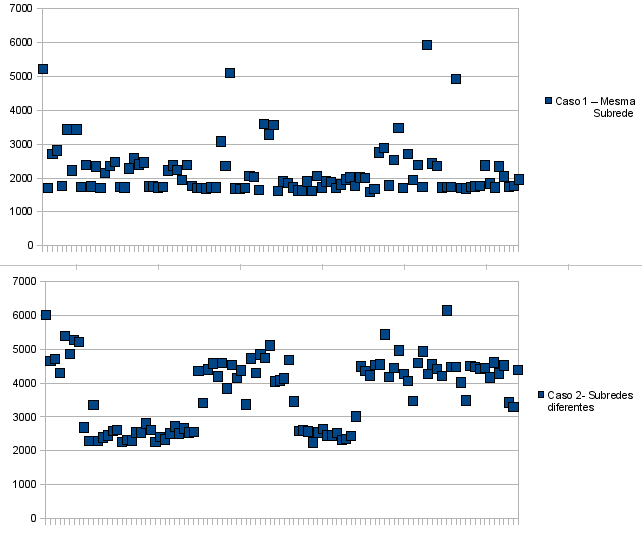
\includegraphics[width=15cm]{consulta.png} 
  \caption{Representação das medições para a consulta.}
  \label{fig:rtt}
\end{figure}

\subsection{Comparação de Desempenho entre TCP e UDP}
Para comparar os resultados de tempo de consulta entre um servidor TCP e outro UDP, vamos colocar os tempos lado a lado:

\textbf{Configuração 1: Mesma Sub-rede}
Médias do tempo de consulta:
- TCP: 1769,16 us
- UDP: 2288,52 us

Desvios padrão:
- TCP: 432,29 us
- UDP: 792,62 us

\textbf{Configuração 2: Sub-redes diferentes}
Médias do tempo de consulta:
- TCP: 9390,89 us
- UDP: 3606,54 us

Desvios padrão:
- TCP: 9758,98 us
- UDP: 1094,37 us


%\begin{figure}[htb]
%  \centering
%  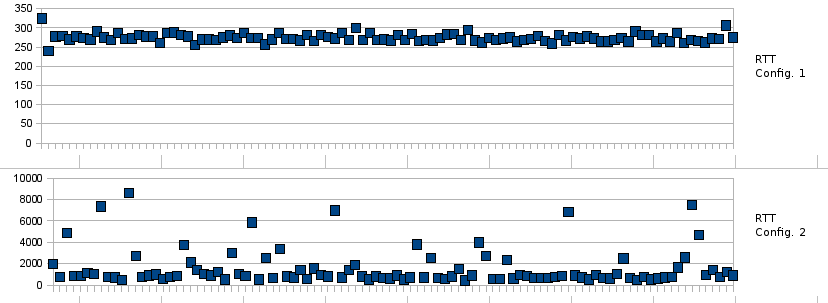
\includegraphics[width=15cm]{rtt.png} 
%  \caption{Representação das medições para o RTT.}
%  \label{fig:rtt}
%\end{figure}

Pode-se verificar a diferença considerável entre os tempos de RTT para as duas configurações. Obviamente, o tempo para abertura da conexão foi maior para a segunda 
configuração, já que os pacotes devem ser transmitidos através de roteadores e enlaces adicionais, como mostrado no resultado do traceroute acima.\\
De modo a comprovar a influência do tráfego na rede, é visível a grande diferença entre os desvios padrão em porcentagem com relação ao valor absoluto.\\


\section{Confiabilidade e Consistência}
Dois pontos a considerar: robustez quanto à comunicação e consistência dos dados.\\
Tentamos fazer todas as verificações de erros possíveis nas funções das bibliotecas de comunicação com o socket, tanto no lado cliente como no servidor. Ainda assim, não conseguimos implementar um importante caso de exceção: notificar e encerrar o cliente quando o servidor "cai".\\
Com relação à consistência dos dados, esta é garantida pela exclusão mútua nas operações de atualização de avaliação.

\section{Conclusão}
Podemos considerar que a aplicação já está totalmente funcional, todas as consultas estão funcionando corretamente, há a garantia da consistência do banco de dados do cinema e a comunicação entre cliente e servidor está boa, exceto no caso em que o servidor cai, deixando o cliente esperando por uma resposta.\\
Por utilizar o protocolo TCP, a comunicação possui todas as suas vantagens, como confiabilidade na transferência de pacotes, controle de fluxo e controle de congestionamento, o que garante uma qualidade maior à aplicação.\\
A análise de tempo também cumpriu com as espectativas, tendo uma média e um desvio padrão mais baixo para redes próximas e valores mais altos para redes mais distantes.\\
Ao fazer a aplicação em C, o nível de abstração não foi muito alto, pois tivemos que tratar muitos detalhes das conexões.\\
Podemos dizer também que fomos felizes ao utilizar um controle de conexões por threads, pois fica mais fácil de controlar do que com processos, já que quando o processo principal termina, todas as threads também terminam, evitando assim processos zumbi, além de ser mais fácil se implementar exclusão mútua de threads, por exemplo, com semáforos ou mutex lock.\\
Nosso servidor de banco de dados de cinema ainda não é um sistema completo e bem acabado, mas já provê uma base sólida para implementar aplicações gráficas e de maior porte, utilizando o servidor como o núcleo da aplicação. Pretendemos, em versões posteriores, melhorar o programa, resolver bugs e talvez, utilizar uma biblioteca gráfica para tornar sua interface mais usável. 

\section{Código Fonte}
\subsection{Makefile}
\begin{verbatim}
# Variáveis
CC = gcc
CC_FLAGS = -ggdb -Wall


# Dependências gerais
all: client server

# Cliente
client: data_access.o internet.o client.o
	$(CC) $(CC_FLAGS) data_access.o internet.o client.o -o client

client.o: client.c data_access.h internet.h defines.h
	$(CC) $(CC_FLAGS) -c client.c

# Servidor
server: data_access.o internet.o server.o
	$(CC) $(CC_FLAGS) data_access.o internet.o server.o -o server

server.o: server.c data_access.h internet.h defines.h
	$(CC) $(CC_FLAGS) -c server.c

# Bibliotecas
data_access.o: data_access.c data_access.h defines.h
	$(CC) $(CC_FLAGS) -c data_access.c

internet.o: internet.c internet.h defines.h
	$(CC) $(CC_FLAGS) -c internet.c


# Relatório (LaTeX)
relatorio:
	pdflatex relatorio.tex

# Clean
clean:
	rm *.o client server *.aux *.toc *.pdf *.log
\end{verbatim}

\subsection{repeat\_client.sh}
\begin{verbatim}
\end{verbatim}

\subsection{arq.in}
\begin{verbatim}
\end{verbatim}

\subsection{client.c}
\begin{verbatim}
\end{verbatim}

\subsection{server.c}
\begin{verbatim}
\end{verbatim}

\subsection{defines.h}
\begin{verbatim}
\end{verbatim}

\subsection{internet.h}
\begin{verbatim}
\end{verbatim}

\subsection{internet.c}
\begin{verbatim}
\end{verbatim}

\subsection{data\_access.h}
\begin{verbatim}
\end{verbatim}

\subsection{data\_access.c}
\begin{verbatim}
\end{verbatim}



%\section{Anexo}
%\begin{figure}[htb]
%  \centering
%  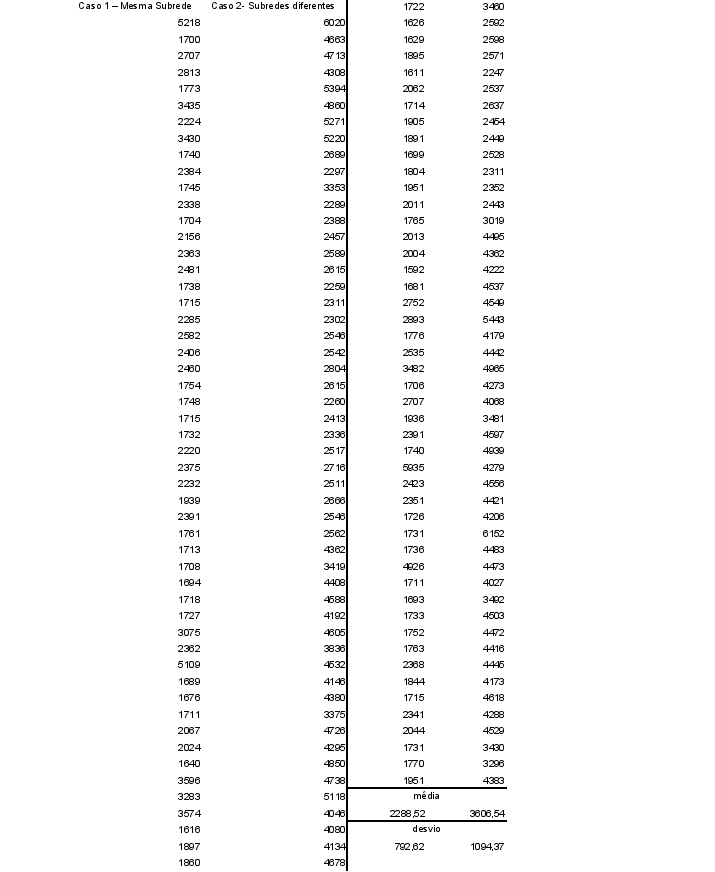
\includegraphics[width=15cm]{medicoes.png} 
%  \caption{Representação das medições para a consulta.}
%  \label{fig:rtt}
%\end{figure}

\begin{thebibliography}{99}
\bibitem{R1} HALL, Brian. Beej's Guide to Network Programming. Disponível em: http://http://beej.us/guide/bgnet/output/html/multipage/index.html.
\end{thebibliography}

\end{document}
